%%%%%%%%%%%%%%%%%%%%%%%%%%%%%%%%%%%%%%%%%
% baposter Landscape Poster
% LaTeX Template
% Version 1.0 (11/06/13)
%
% baposter Class Created by:
% Brian Amberg (baposter@brian-amberg.de)
%
% This template has been downloaded from:
% http://www.LaTeXTemplates.com
%
% License:
% CC BY-NC-SA 3.0 (http://creativecommons.org/licenses/by-nc-sa/3.0/)
%
%%%%%%%%%%%%%%%%%%%%%%%%%%%%%%%%%%%%%%%%%

%----------------------------------------------------------------------------------------
%	PACKAGES AND OTHER DOCUMENT CONFIGURATIONS
%----------------------------------------------------------------------------------------

\documentclass[landscape,archE,fontscale=0.29]{baposter} % Adjust the font scale/size here

%%% Start of code to add %%%
\usepackage{etoolbox}
\patchcmd\thebibliography
    {\labelsep}
    {\labelsep\itemsep=0pt\relax}
    {}
    {\typeout{Couldn't patch the command}}
%%% End of code to add %%%

\usepackage{url}
\usepackage{lipsum}

\usepackage{graphicx} % Required for including images
\graphicspath{{figures/}} % Directory in which figures are stored

\usepackage{amsmath} % For typesetting math
\usepackage{amssymb} % Adds new symbols to be used in math mode

\usepackage{booktabs} % Top and bottom rules for tables
\usepackage{enumitem} % Used to reduce itemize/enumerate spacing
\usepackage{palatino} % Use the Palatino font
\usepackage[font=small,labelfont=bf]{caption} % Required for specifying captions to tables and figures

\usepackage{multicol} % Required for multiple columns
\usepackage{vwcol} % variable-width mul­ti­ple text columns
\setlength{\columnsep}{0.5em} % Slightly increase the space between columns
\setlength{\columnseprule}{0mm} % No horizontal rule between columns

\usepackage{tikz} % Required for flow chart
\usetikzlibrary{shapes,arrows} % Tikz libraries required for the flow chart in the template

\newcommand{\compresslist}{ % Define a command to reduce spacing within itemize/enumerate environments, this is used right after \begin{itemize} or \begin{enumerate}
\setlength{\itemsep}{1pt}
\setlength{\parskip}{0pt}
\setlength{\parsep}{0pt}
}

\definecolor{lightblue}{rgb}{0.145,0.6666,1} % Defines the color used for content box headers

% my macros
\newcommand{\myv}{\vspace{-1mm}}


\begin{document}

\begin{poster}
{
headerborder=closed, % Adds a border around the header of content boxes
colspacing=1em, % Column spacing
bgColorOne=white, % Background color for the gradient on the left side of the poster
bgColorTwo=white, % Background color for the gradient on the right side of the poster
borderColor=lightblue, % Border color
headerColorOne=black, % Background color for the header in the content boxes (left side)
headerColorTwo=lightblue, % Background color for the header in the content boxes (right side)
headerFontColor=white, % Text color for the header text in the content boxes
boxColorOne=white, % Background color of the content boxes
textborder=roundedleft, % Format of the border around content boxes, can be: none, bars, coils, triangles, rectangle, rounded, roundedsmall, roundedright or faded
eyecatcher=true, % Set to false for ignoring the left logo in the title and move the title left
headerheight=0.13\textheight, % Height of the header
headershape=roundedright, % Specify the rounded corner in the content box headers, can be: rectangle, small-rounded, roundedright, roundedleft or rounded
headerfont=\Large\bf\textsc, % Large, bold and sans serif font in the headers of content boxes
%textfont={\setlength{\parindent}{1.5em}}, % Uncomment for paragraph indentation
linewidth=2pt % Width of the border lines around content boxes
}
%----------------------------------------------------------------------------------------
%	TITLE SECTION
%----------------------------------------------------------------------------------------
%
%% {
\includegraphics[height=10em]{img/UniversityOfWaterloo_logo_vert_rgb.png}} % First university/lab logo on the left
{
\includegraphics[height=7.5em]{img/Cheriton_Logo.pdf}} % First university/lab logo on the left
{\bf\textsc{Univenture: A Quest to Greatness}\vspace{0.1em}} % Poster title
{\vspace{-2mm}
\textsc{Xu Cui, Xinan Yan, and
    Ivens Portugal \\ David R. Cheriton School of Computer Science}} % Author names and institution
%% {\includegraphics[height=4em]{logo.png}} % Second university/lab logo on the right

%----------------------------------------------------------------------------------------
%	OBJECTIVES
%----------------------------------------------------------------------------------------

\headerbox{Background}{name=background, column=0, row=0, height=0.70}{
%% Cloud allows sharing which increases resource utilization that in turn reduces costs. However, with increased utilization there is also reduced isolation between tenants. This is especially problematic for cloud storage systems which are highly sensitive to performance interference. Since cloud storage is often the performance bottleneck in cloud application, a lack of performance isolation can lead to unpredictable application latencies.
\textbf{Common Problems Among First-Year University Students}
\myv
\begin{itemize}
\item Suicide in colleges has become a serious problem. \cite{kenedy2013}
\item Alcohol and drug abuse is common among university students. \cite{tamburri2013}
\item Many students are heavily stressed due to overwhelming responsibilities.
\item Students who live on their own for the first time may have social anxiety and feel isolated.
\end{itemize}

\textbf{Current Solutions}
\myv
\begin{itemize}
\item Universities provide free counselling services.
\item Universities and non-profit organizations host various workshops and seminars.
\item Upper-year students provide mentorship to junior students.
\item These resources are limited. For instance, The Ryerson University has 14 counsellors to work with a student body with a population of 28,300. \cite{Lunau2012}
\item Many students who are in need of support may not be aware of these services.
\end{itemize}

%% \begin{itemize}\compresslist
%% \item[--] \scriptsize{[1] Nathan Farrington and Alexey Andreyev, Facebook's Data
  %% Center Network Architecture.}
%% \item[--] \scriptsize{[2] Greg Lindem, Make Data Useful,
  %% \url{http://www.scribd.com/doc/4970486/Make-Data-Useful-by-Greg-Linden-Amazon-com}.}
%% \end{itemize}
\vspace{0.2em} % When there are two boxes, some whitespace may need to be added if the one on the right has more content
}


\headerbox{Univenture: A Quest To Greatness}{name=microfuge,column=1,span=2,row=0, height=0.33}{
  \begin{minipage}{0.7\linewidth}
    %% \vspace{0.5em}
    \myv
    \myv
    A massive-multiplayer-virtual-role-playing game designed for mobile devices.

    \begin{itemize}\compresslist
    \item University students role-play as \textbf{Adventurers} (first-year students) or \textbf{Guardians} (upper-year students) in Univenture.
    \item Players earn both in-game and real-life \textbf{rewards} by completing in-game quests.
    \item \textbf{Quests} not only facilitate player activities which are good for mental health, but give students motivation to overcome real-life challenges.
    \item Univenture features a well-thought virtual environment to facilitate mentorship and reaching out.
    \end{itemize}


  \end{minipage}
  \begin{minipage}{0.3\linewidth}
    \begin{center}
      
\includegraphics[scale=0.10]{img/univenture_main.jpg}
      \captionof{figure}{The Univenture App}
    \end{center}
  \end{minipage}



\vspace{0.2em} % When there are two boxes, some whitespace may need to be added if the one on the right has more content
}


\headerbox{Mental Health and Gameplay}{name=cache, column=1, span=2, below=microfuge, above=bottom}{
  %% \textbf{DLC} offers adaptive deadline-aware caching.
  %% \myv \myv \myv
  \begin{minipage}{0.26\linewidth}
    \begin{center}
      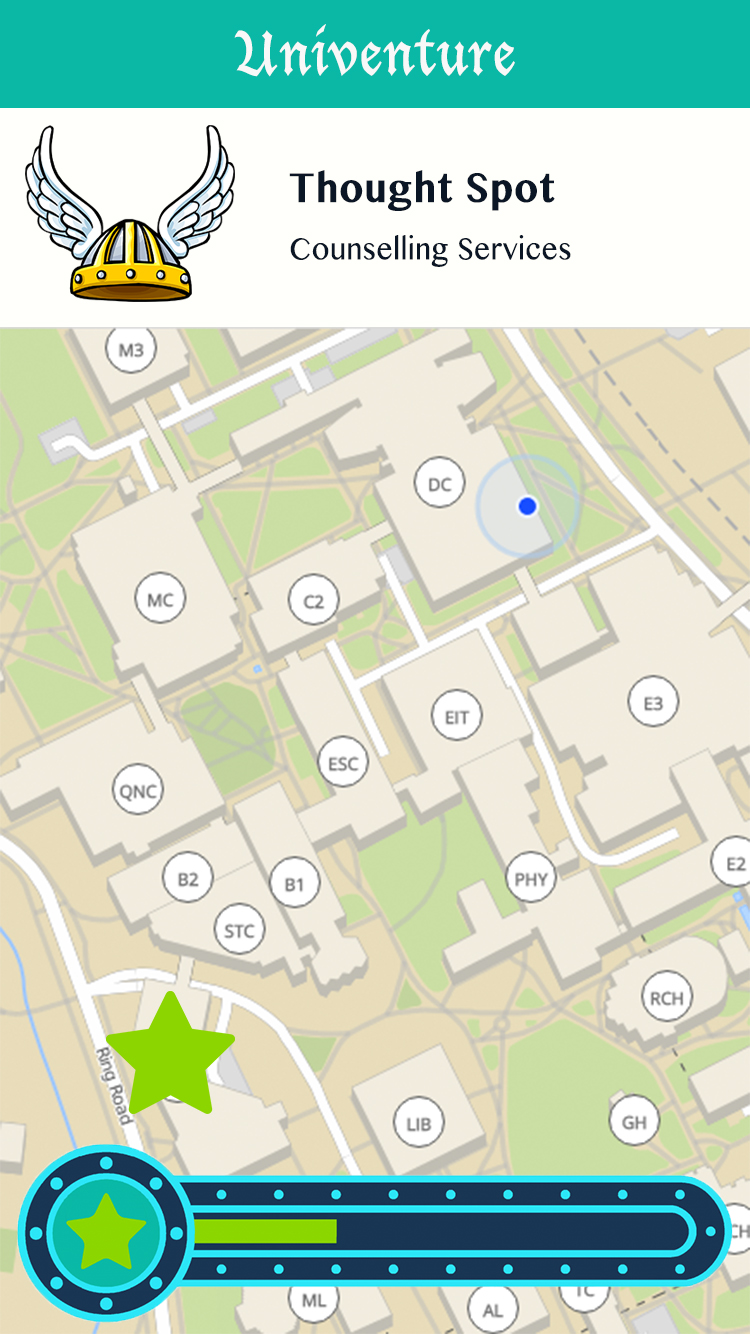
\includegraphics[scale=0.10]{img/discovery_quest.jpg}
      \captionof{figure}{A Discovery Quest}
    \end{center}
  \end{minipage}
  \begin{minipage}{0.72\linewidth}
    \textbf{Problem 1}: New university students do not know which local resources are available to assist them with their mental health problems.
    \\
    \textbf{Solution}:
    \myv \myv
    \begin{itemize} \compresslist
    \item Univenture introduces \textbf{exploration quests}.
    \item In exploration quests, adventurers are asked to visit various locations reported by \textbf{Thought Spot}.
    \item Thought Spot is a web application built by \textbf{CAMH} (Canada's Mental Health Hospital) that contains a database of health service resources for students.
    \item Furthermore, Univenture allows students to directly contribute to Thought Spot by sending the geo-coordinates and auxiliary information of helpful locations to Thought Spot through an in-game interface.
    \end{itemize}
  \end{minipage}

  \begin{minipage}{0.72\linewidth}
    \vspace{2.5mm}
    \textbf{Problem 2}: Many students struggle with academic performance due to the major changes introduced by the transition from high school to university. This leads to anxiety and stress.
    \\
    \textbf{Solution}:
    \myv \myv
    \begin{itemize} \compresslist
    \item Univenture introduces course dungeons.
    \item Univenture asks players to provide the courses they are taking and the deliverables for each course, and generates a group of mini-monsters for each course.
    \item Students defeat these mini-monsters while they are progressing through the term.
    \item Univenture, in turn, celebrates academic achievement by rewarding experience points to the player.
    \item This gamification of academic progression  reminds the students to celebrate their intermediate progress and also motivates the students to continue their journey.
    \end{itemize}
  \end{minipage}
  \begin{minipage}{0.26\linewidth}
    \begin{center}
      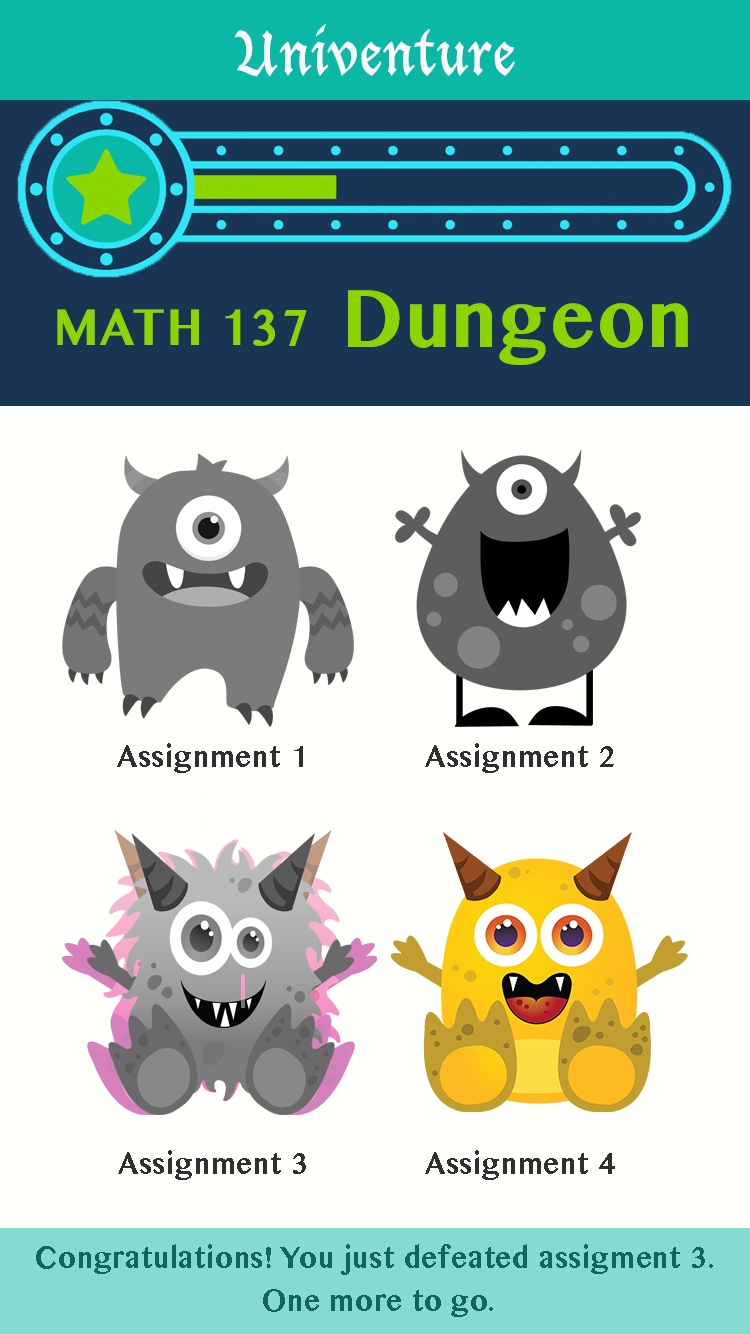
\includegraphics[scale=0.10]{img/mini_moster.jpg}
      \captionof{figure}{A Dungeon}
    \end{center}
  \end{minipage}

}

%% \headerbox{Additional Features}{name=scheduler, column=3, span=1,  bottomaligned=background}{
%%   \begin{itemize}
%%   \item Univenture has leaderboard rankings of Adventurers and Guardians according to the their points which, in turn, promotes players to engage in both in-game and social activities.
%%   \item Univenture has a support group feature such that students can discuss potential mental and health issues as well as the solutions to them.
%%   \item Univenture allows adventurers to send out stress signs to guardians which indicates that he/she would like a one-to-one help from other experienced players.
%%   \end{itemize}
%%   %% \myv \myv \myv \myv \myv \myv \myv \myv
%%   \begin{center}
%%     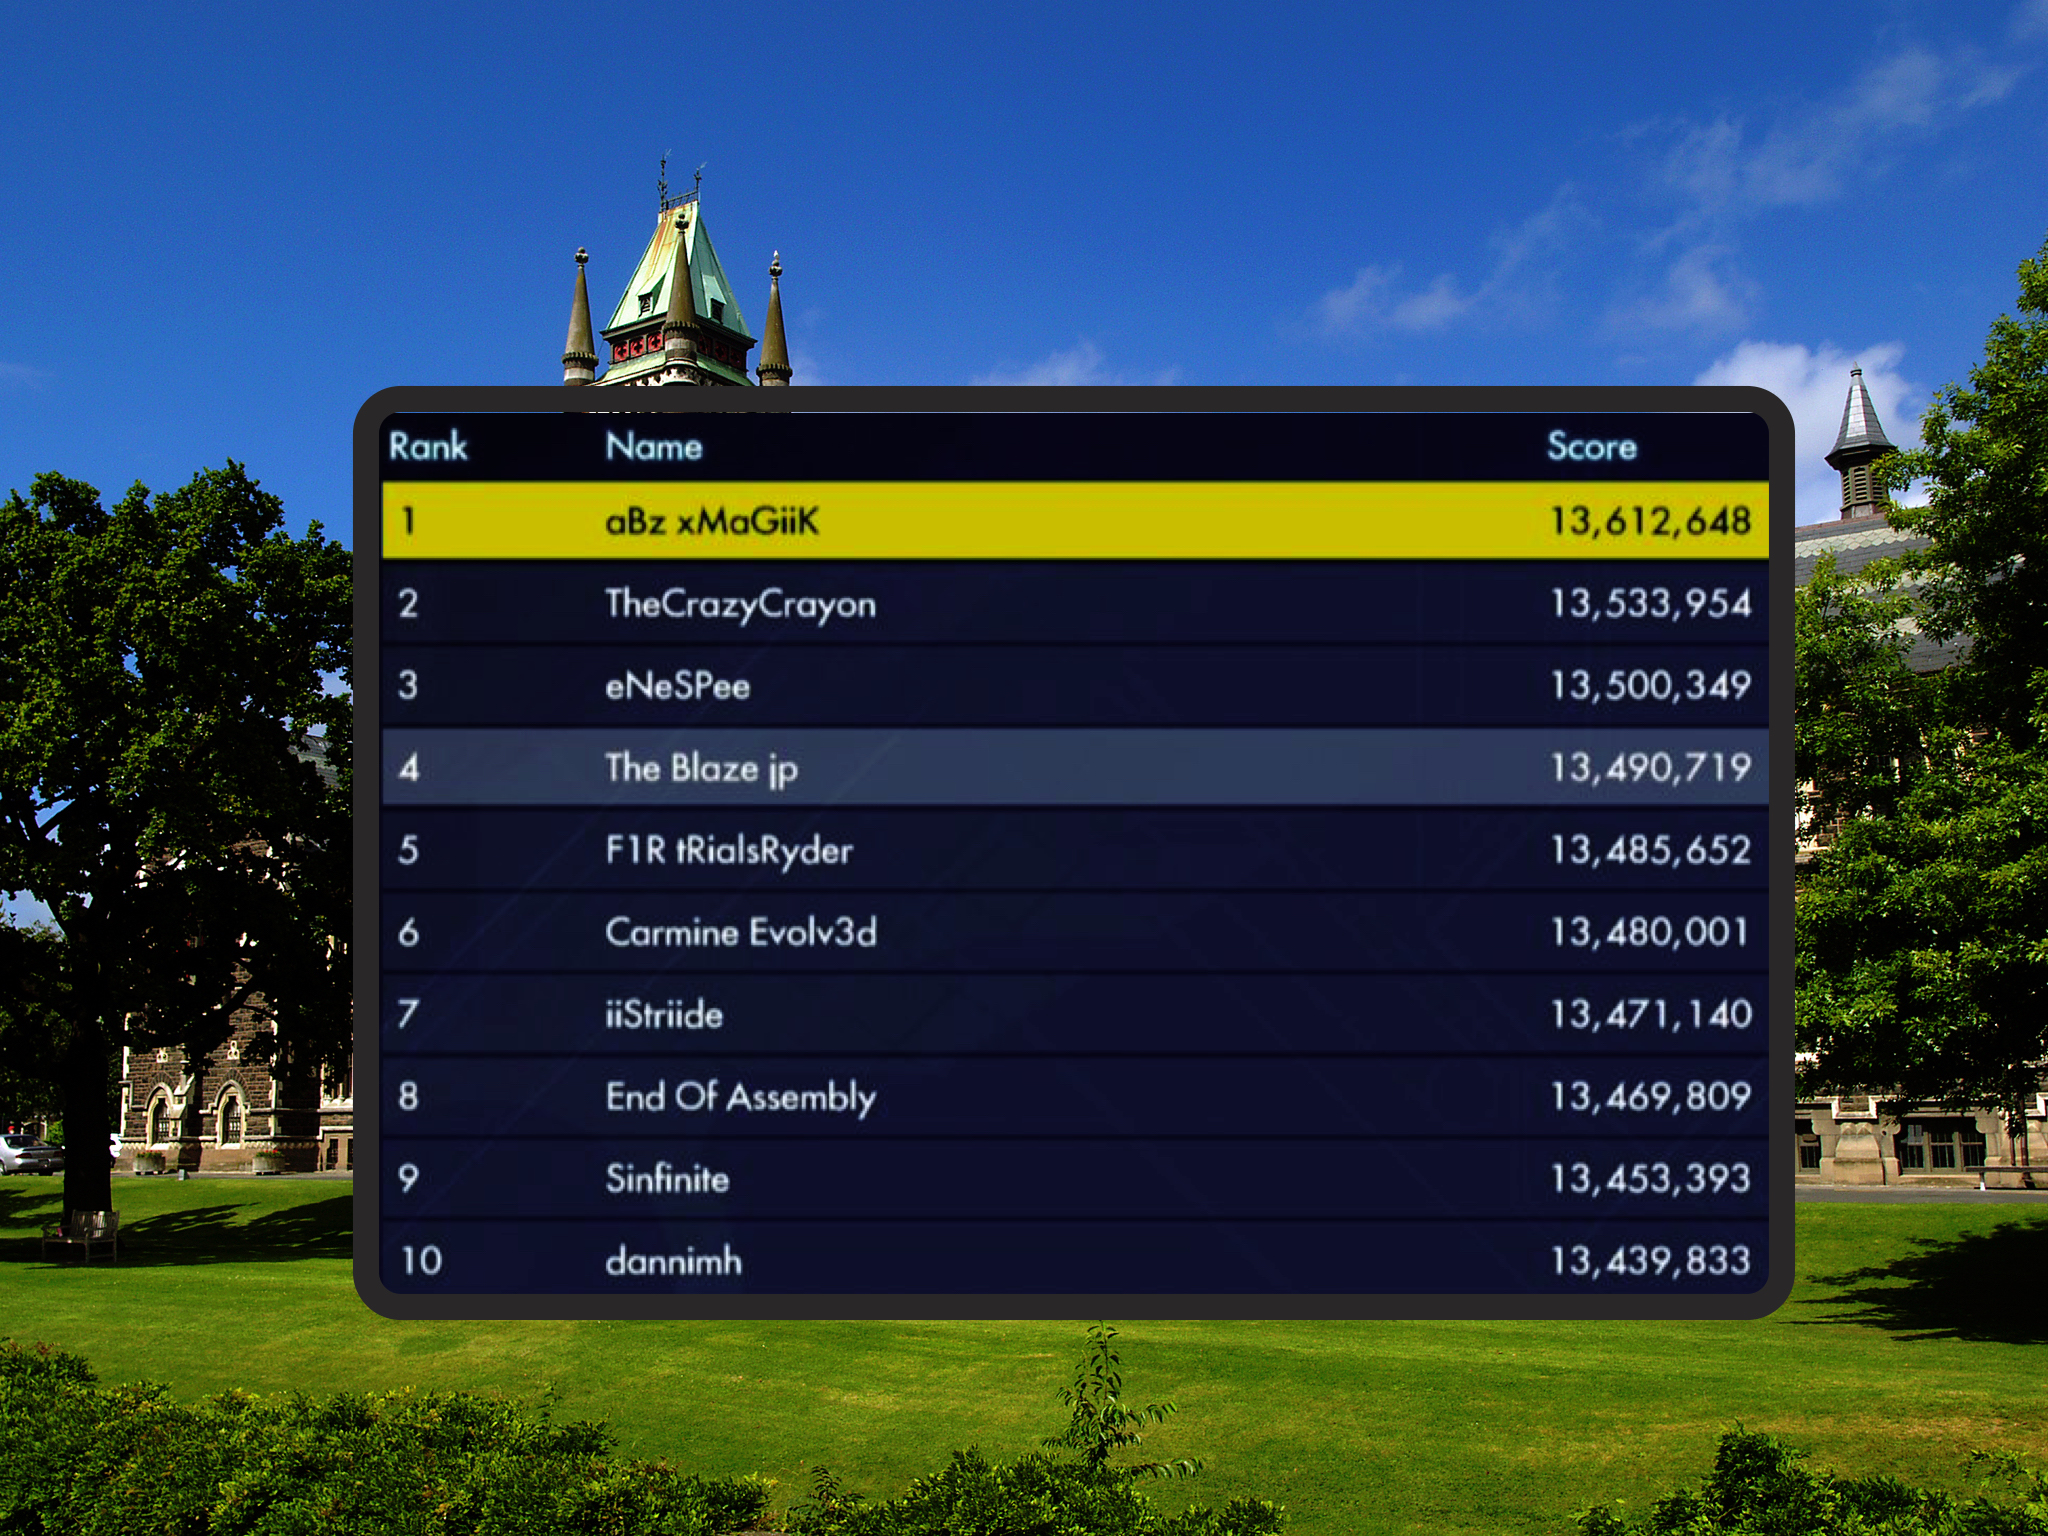
\includegraphics[scale=0.10]{img/Univenture_Leaderboard.jpg}
%%     \captionof{figure}{A Leaderboard}
%%   \end{center}
%% }

%% \headerbox{References}{name=reference, column=0,below=background, above=bottom}{
%%   \renewcommand{\section}[2]{\vskip 0.05em%
%%   } % Get rid of the default ``References'' section title

%%   \nocite{*} % Insert publications even if they are not cited in the poster
%%   \small{ % Reduce the font size in this block
%%     \bibliographystyle{unsrt}
%%     \bibliography{g4h} % Use sample.bib as the bibliography file
%%   }
%% }  %% Additional Features

\headerbox{Player Avatar and Rewards}{name=scheduler, column=3, span=1,  bottomaligned=background}{
  \textbf{Problem 3}: Many students are overwhelmed by the large number of academic deadlines in universities. Therefore, they may lose their interest and motivation.
  \\
  \textbf{Solution}:
  \myv \myv
  \begin{itemize} \compresslist
    \item Univenture keeps players motivated by constantly celebrating and rewarding their progress.
    \item Univenture provides both virtual and real-life rewards as stimuli to promote player adherence.
    \item Univenture allows players to spend their in-game experience points to improve their avatar and to purchase titles and badges.
    \item Univenture also provides real-world rewards such as coupons from supporting companies.
    \item Students may even have their accomplishments shown on their transcripts.
  \end{itemize}
  %% \myv \myv \myv \myv \myv \myv \myv \myv
  \begin{minipage}{0.47\linewidth}
    \begin{center}
      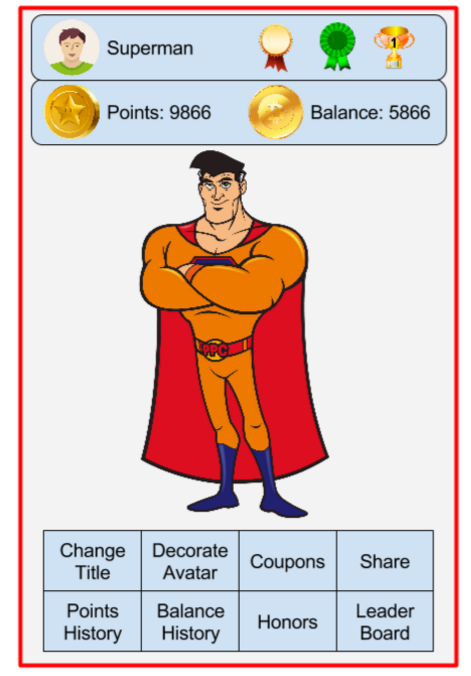
\includegraphics[scale=0.15]{img/avatar.png}
      \captionof{figure}{Player Avatar}
    \end{center}
  \end{minipage}
  \begin{minipage}{0.47\linewidth}
    \begin{center}
    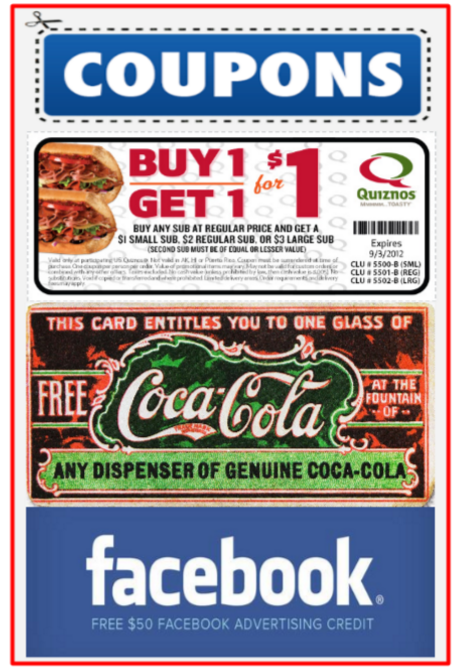
\includegraphics[scale=0.15]{img/rewards}
    \captionof{figure}{Game Rewards}
    \end{center}
  \end{minipage}
  %% \begin{center}
    %% 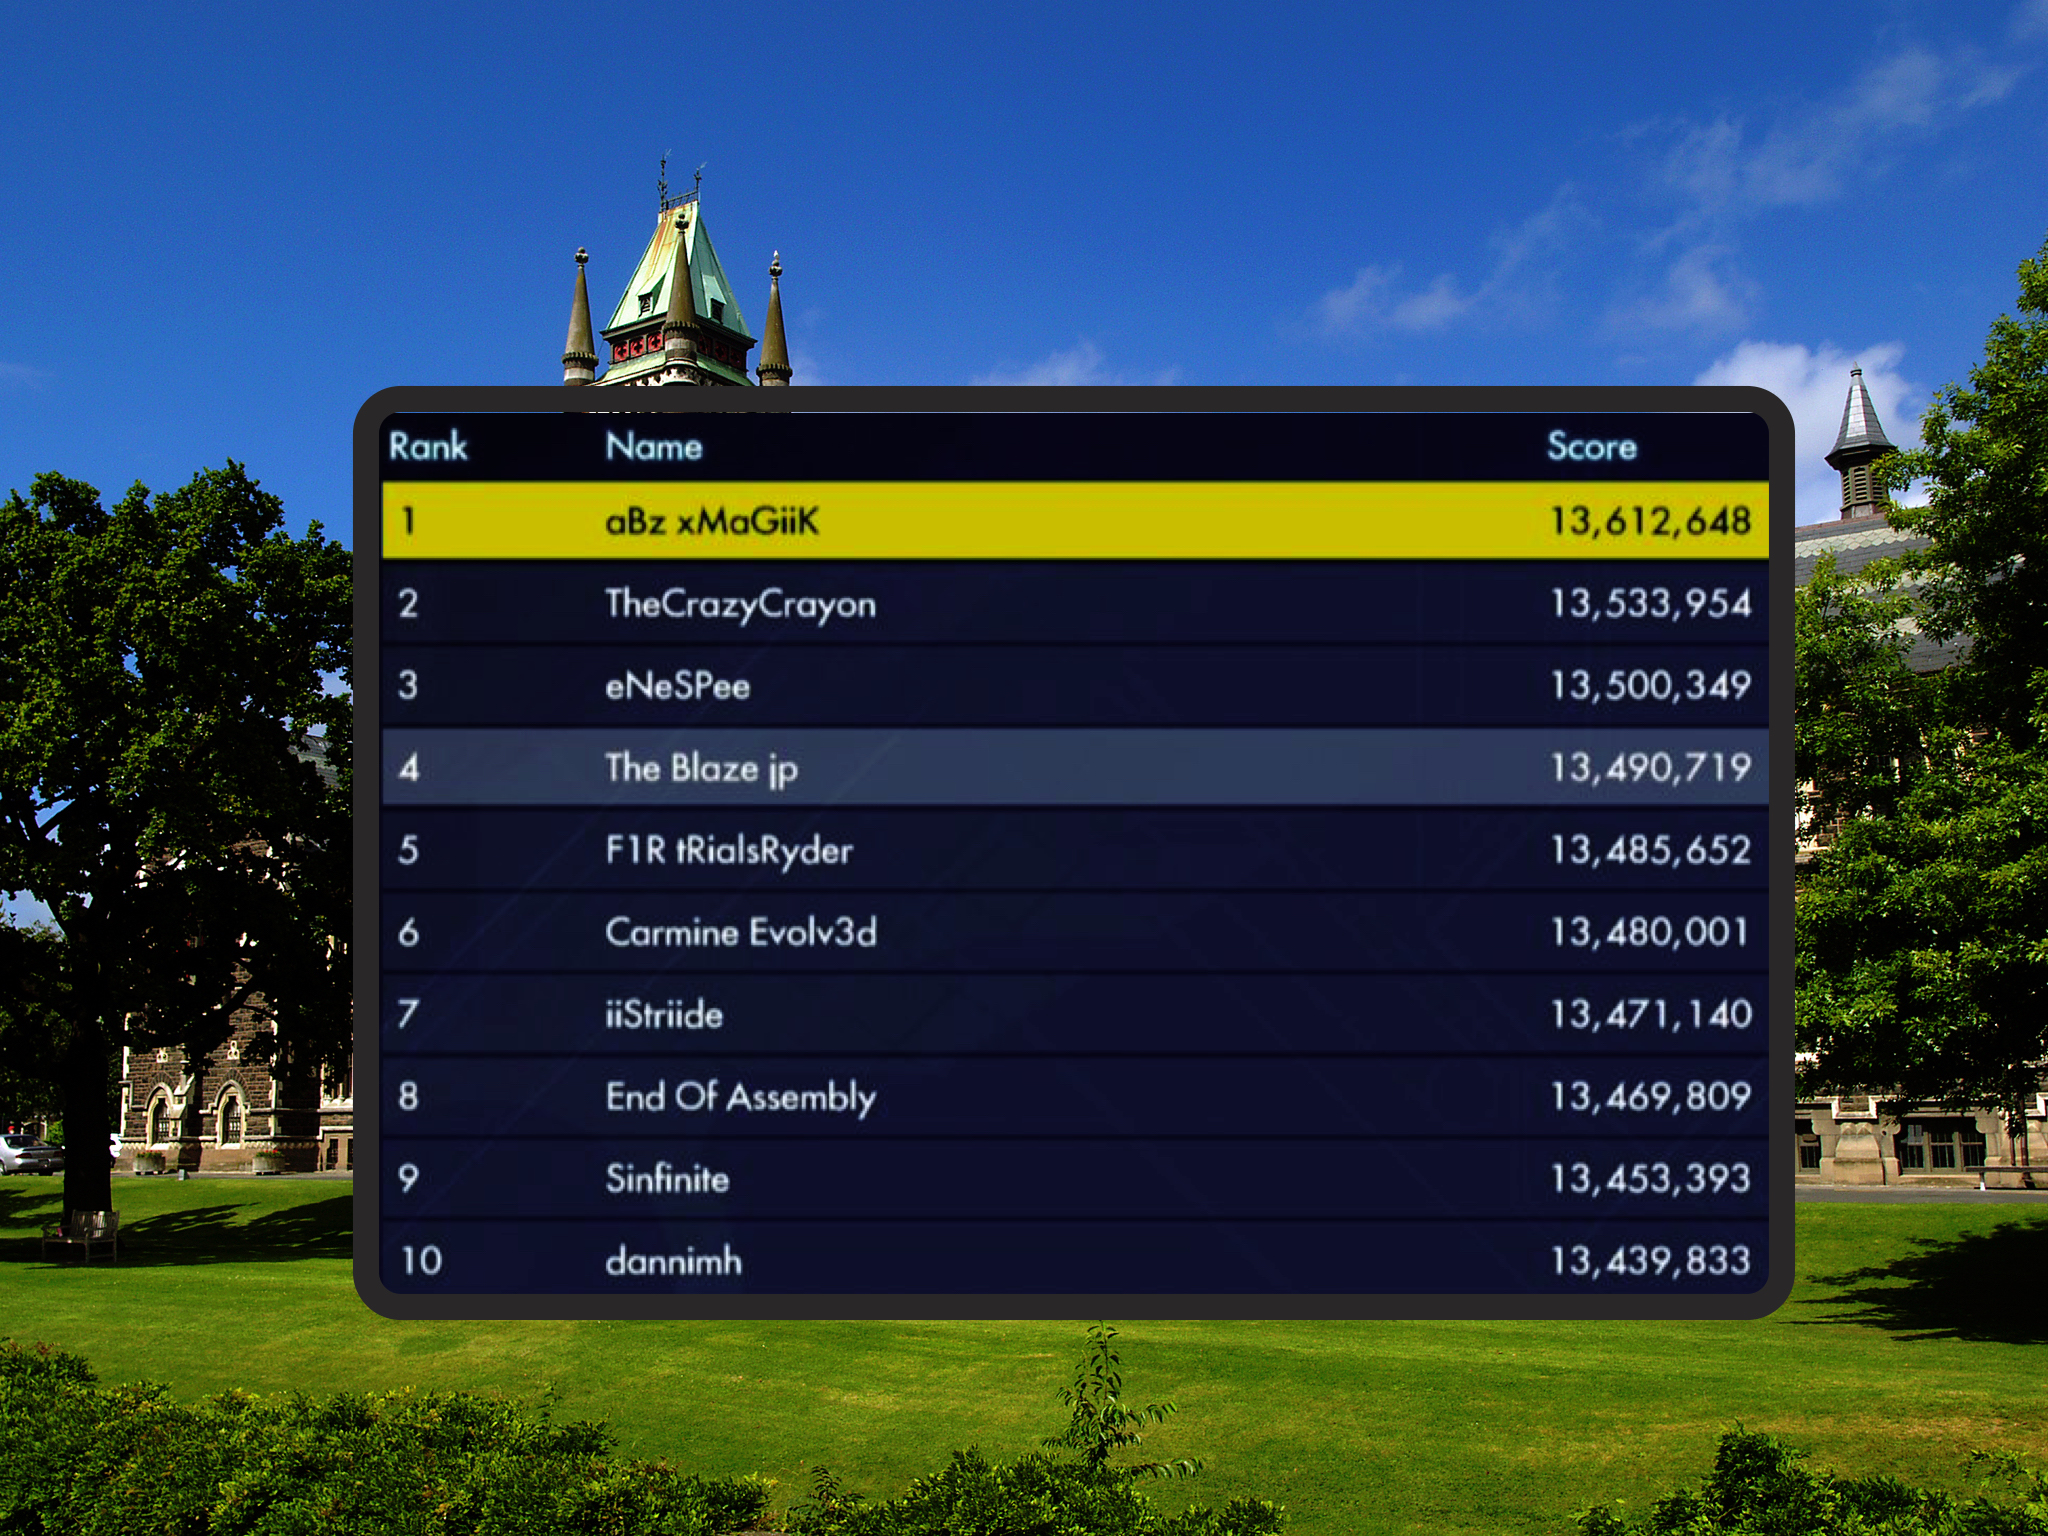
\includegraphics[scale=0.10]{img/Univenture_Leaderboard.jpg}
    %% \captionof{figure}{A Leaderboard}
  %% \end{center}
}

\headerbox{References}{name=reference, column=0,below=background, above=bottom}{
  \renewcommand{\section}[2]{\vskip 0.05em%
  } % Get rid of the default ``References'' section title

  \nocite{*} % Insert publications even if they are not cited in the poster
  \small{ % Reduce the font size in this block
    \bibliographystyle{unsrt}
    \bibliography{g4h} % Use sample.bib as the bibliography file
  }
}

%% \headerbox{Player Avatar and Rewards}{name=performance, column=1, span=2,below=background, above=bottom}{
%%   \begin{minipage}{0.24\linewidth}
%%     \begin{center}
%%       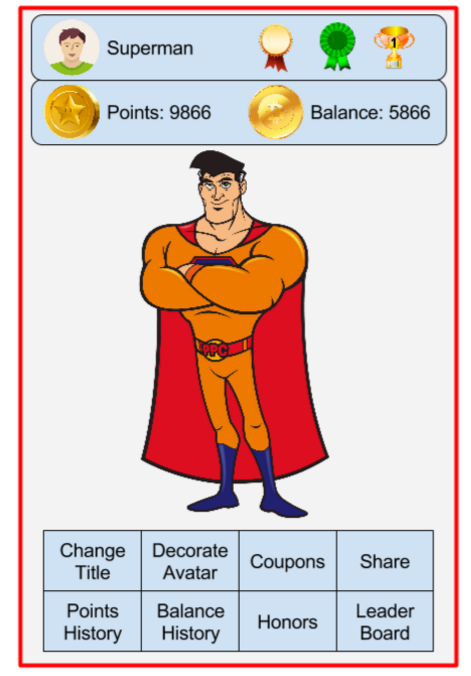
\includegraphics[scale=0.15]{img/avatar.png}
%%       \captionof{figure}{Player Avatar}
%%     \end{center}
%%   \end{minipage}
%%   \begin{minipage}{0.24\linewidth}
%%     \begin{center}
%%     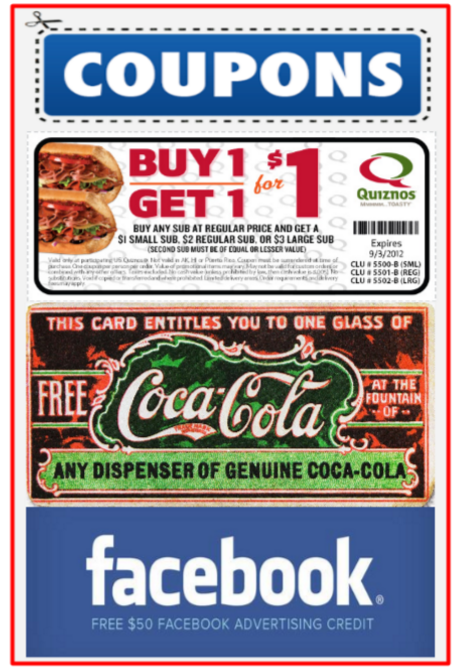
\includegraphics[scale=0.15]{img/rewards}
%%     \captionof{figure}{Game Rewards}
%%     \end{center}
%%   \end{minipage}
%%   \begin{minipage}{0.52\linewidth}
%%     \begin{itemize}\compresslist
%%       \vspace{0.1mm}
%%     \item Univenture provides both virtual and real-life rewards as stimuli to promote player adherence.
%%     \item Univenture allows players to spend their in-game experience points to improve their avatar and to purchase titles and badges.
%%     \item Univenture also provides real-world rewards such as coupons from supporting companies.
%%     \item Students may even have their accomplishments shown on their transcripts.
%%     \end{itemize}
%%   \end{minipage}
%% }
\headerbox{Conclusion}{name=conclusion, column=3,below=background, above=bottom}{
  \vspace{0.2em}
  \begin{itemize}
  \item Univenture aims to address mental problems among first-year university students.
  \item Univenture allows students to take university life as an adventure and to learn to embrace its challenges.
  \item Univenture builds a strong connection between the gameplay and university life to improve mental resilience of the first year university students.
  \end{itemize}
}
\end{poster}

\end{document}
